\documentclass[journal]{IEEEtran}
\usepackage{amsmath, amsfonts, graphicx, listings, xcolor, float, caption}

\definecolor{codegreen}{rgb}{0,0.6,0}
\definecolor{codegray}{rgb}{0.5,0.5,0.5}
\definecolor{codepurple}{rgb}{0.58,0,0.82}
\definecolor{backcolour}{rgb}{0.95,0.95,0.92}

\lstdefinestyle{mystyle}{
    backgroundcolor=\color{backcolour},   
    commentstyle=\color{codegreen},
    keywordstyle=\color{magenta},
    numberstyle=\tiny\color{codegray},
    stringstyle=\color{codepurple},
    basicstyle=\ttfamily\footnotesize,
    breakatwhitespace=false,         
    breaklines=true,                 
    captionpos=b,                    
    keepspaces=true,                 
    numbers=left,                    
    numbersep=5pt,                  
    showspaces=false,                
    showstringspaces=false,
    showtabs=false,                  
    tabsize=2
}

\lstset{style=mystyle}

\graphicspath{ {./images/} }

\title{Lab 9: Higher Order IIR Filter Design and Implementation}
\author{
    \IEEEauthorblockN{Argenis Aquino, Rachel DuBois, Diego Lopez, Jonathan Sumner \\}
    \IEEEauthorblockA{
        Department of Engineering Technology, Rochester Institute of Technology\\
        1 Lomb Memorial Drive, Rochester NY, 14623, United States of America \\}
}

\begin{document}
\maketitle

\begin{abstract}
    This lab focused on designing higher order Infinite Impulse Response (IIR) filters using MATLAB and implementing both Direct Form and Second Order Section (SOS) realizations on the Arduino platform. The goal was to gain practical experience with digital filter design, quantization, and implementation in embedded systems. MATLAB was used to design filters, simulate frequency response, and generate coefficients for Arduino deployment.
\end{abstract}

\section{Introduction}
\IEEEPARstart{D}{igital} filters are a fundamental component in signal processing systems. MATLAB was used to design high-order IIR filters using various methods including Butterworth and Chebyshev designs. These filters were implemented on an Arduino to allow hands-on experience in comparing theoretical filter behavior with real-world performance under finite word length constraints. The lab was divided into parts focused on filter design, implementation, and analysis.

MATLAB was used to design 5th and 7th order lowpass and highpass filters, including Butterworth and Chebyshev types, with specified cutoff frequencies and ripple parameters. Filter coefficients were quantized and transferred to Arduino C code. Filters were tested with impulse signals and real-time audio, and the output was analyzed in MATLAB to evaluate filter performance.

\section{Results}
A 5th order Butterworth lowpass filter with a cutoff at 12 BPM was designed and implemented. This filter was expected to have a smooth frequency response with no ripple in the passband.

\begin{figure}[H]
    \centering
    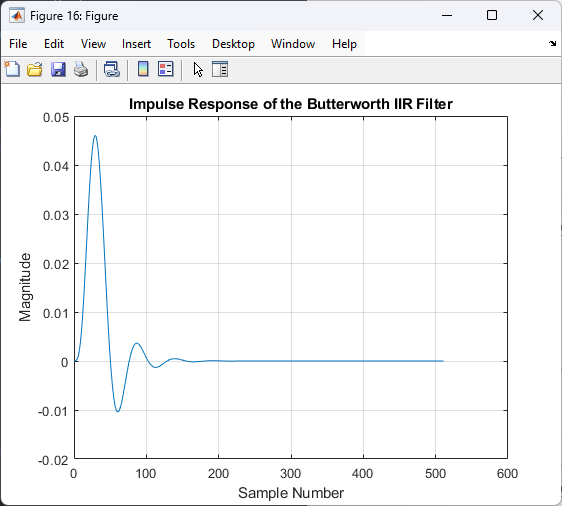
\includegraphics[width=5cm]{5thOrderButterworthImpulse.png}
    \caption{Butterworth Frequency Response (0–50 BPM)}
    \label{fig:butter_impulse}
\end{figure}

Next, a 5th order Chebyshev highpass filter with a 50 BPM cutoff frequency was created. The Chebyshev filter was designed with a ripple of 0.5 dB in the passband, which is a characteristic feature of Chebyshev filters. The frequency response was expected to have a steeper roll-off compared to the Butterworth filter, with some ripple in the passband.

\begin{figure}[H]
    \centering
    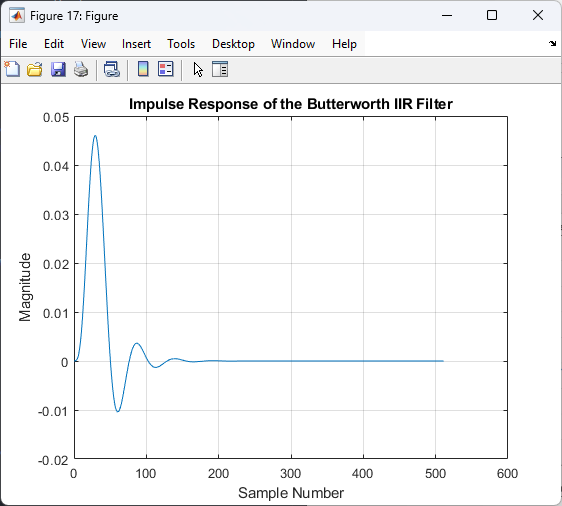
\includegraphics[width=\linewidth]{5thOrderChebyImpulse.png}
    \caption{Chebyshev Frequency Response (0–50 BPM)}
    \label{fig:cheby_impulse}
\end{figure}

A 7th order Chebyshev lowpass filter was then evaluated. It exhibited signs of instability such as unbounded oscillation, highlighting the limitations of direct form implementation for high-order IIR filters.

To address this, the same 7th order filter was implemented using Second Order Sections (SOS). MATLAB’s \texttt{IIR\_Designer} generated the required coefficients and gain values. These were copied into the Arduino sketch, and the impulse response was captured in MATLAB. The SOS implementation maintained stability and matched the theoretical design.

\begin{figure}[H]
    \centering
    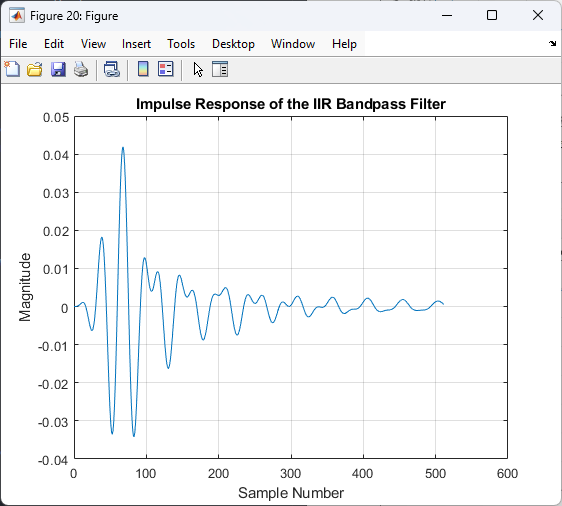
\includegraphics[width=\linewidth]{BandpassSOSImpulse.png}
    \caption{IIR Bandpass Filter Impulse Response}
    \label{fig:band_pass_sos_impulse}
\end{figure}

A bandpass filter was then created using the SOS approach with a 5th order Chebyshev filter spanning 12–25 BPM. The filter was tested using an impulse input, and the resulting impulse and frequency responses confirmed that the filter passed signals in the target band while attenuating others.

To further validate the bandpass filter, a test vector of sinusoidal signals at 5, 10, 15, 20, 30, and 70 BPM was input. The Arduino-filtered output showed attenuation for frequencies outside the passband and accurate passage of frequencies within 12–25 BPM.

\begin{figure}[H]
    \centering
    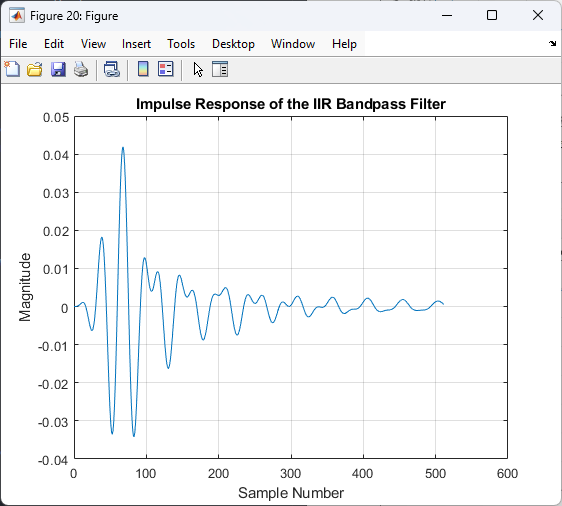
\includegraphics[width=\linewidth]{BandpassSOSImpulse.png}
    \caption{IIR Bandpass Filter using Second Order Stages}
    \label{fig:band_pass_sos}
\end{figure}

\section{Analysis}
By finding the magnitude and the frequency of the filter in breaths per minute (BPM), the Butterworth filter data was successfully plotted and analyzed.

\begin{equation}
    MAG_{dB} = 20 \cdot \log_{10} \left( \lvert Y \rvert \right)
\end{equation}

where $Y$ is the impulse response.

\begin{equation}
    Freq_{Hz} = \frac{n \cdot f_s}{N}
\end{equation}

where $n$ is the index of the frequency bin, $f_s$ is the sampling frequency, and $N$ is the total number of samples.

To convert to breaths per minute (BPM), the frequency in Hz can be multiplied by 60.

Using these equations, the frequency response of the Butterworth filter was plotted. The results showed that the filter effectively isolated the desired frequency range, confirming its design specifications.

\begin{figure}[H]
    \centering
    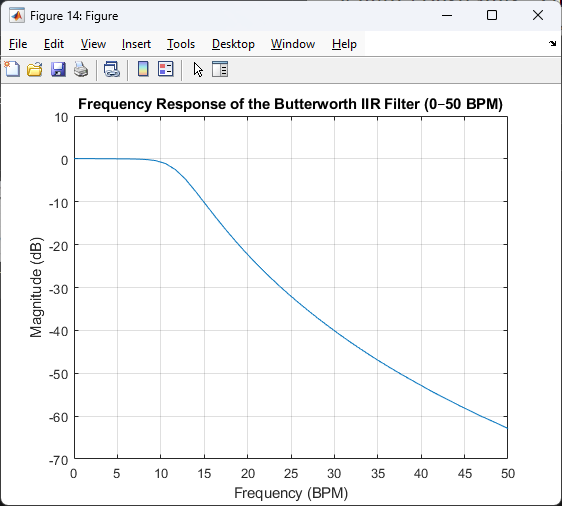
\includegraphics[width=\linewidth]{5thOrderButtwerworthFrequency.png}
    \caption{IIR Butterworth Filter using SOS Frequency Response}
    \label{fig:band_pass_sos_freq}
\end{figure}

The same equations were applied to the Chebyshev lowpass filter, and the results were compared. The Chebyshev filter exhibited a steeper roll-off and ripple in the passband, consistent with its design characteristics.
The frequency response of the Chebyshev filter was also plotted, confirming its design specifications.

\begin{figure}[H]
    \centering
    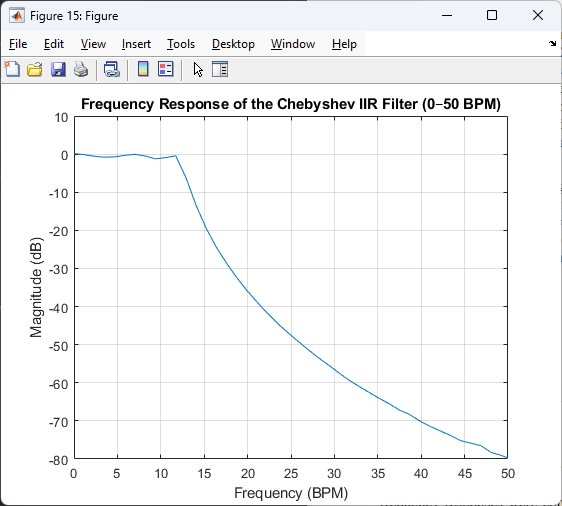
\includegraphics[width=\linewidth]{5thOrderChebyFrequency.png}
    \caption{5th Order Chebyshev Lowpass Filter Frequency Response}
    \label{fig:cheby_low_freq}
\end{figure}

In order to detect breathing rates above 25 BPM a highpass filter was designed. The filter was created with a 5th order Chebyshev design, 25 BPM cutoff frequency, and a ripple of 1.0 dB. The filter was plotted using the the magnitude and frequency equations. The results showed that the filter effectively attenuated frequencies below 25 BPM, confirming its design specifications.

\begin{figure}[H]
    \centering
    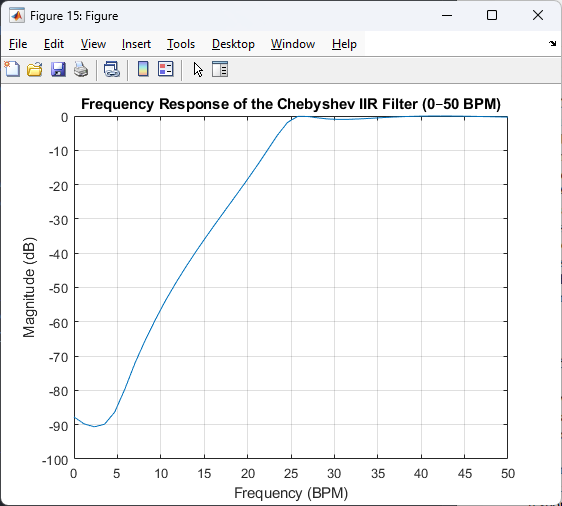
\includegraphics[width=\linewidth]{5thOrderChebyHighpassFrequency.png}
    \caption{IIR Bandpass Filter using Second Order Stages}
    \label{fig:cheby_high_freq}
\end{figure}

This filter proved successfull as it can be seen that when the BPM reached 25, the output was attenuated.

When implemented in the Direct Form, high order IIR filters exhibited instability, leading to oscillations and unbounded output. This was particularly evident in the 7th order Chebyshev filter, which was designed with a ripple of 0.5 dB. The SOS implementation resolved these issues by breaking the filter into smaller, stable sections, allowing for accurate real-time processing on the Arduino.

\begin{figure}[H]
    \centering
    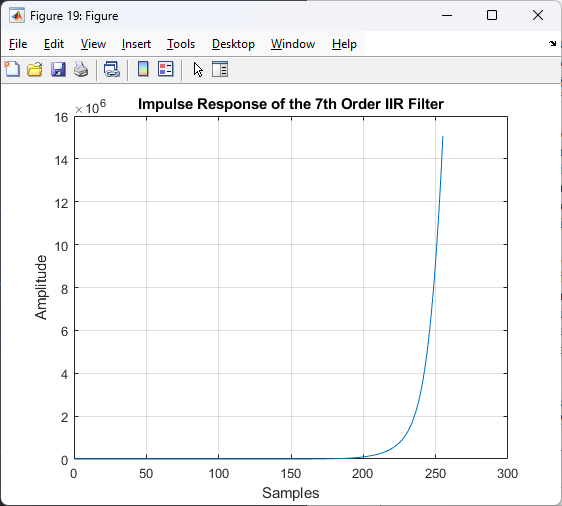
\includegraphics[width=\linewidth]{7thOrderChebyImpulse.png}
    \caption{7th Order Chebyshev Filter Impulse Response}
    \label{fig:7th_cheby_high_impulse}
\end{figure}

The plot shows the impulse response of the 7th order Chebyshev filter, which was unstable in direct form.

One way of implementing higher order IIR filters and maintain stability is to use the Second Order Stages method. Here the filter is broken into smaller second order stages. This can be done by using the transfer function:

\begin{equation}
    H(z) = \frac{\sum_{k=0}^{M} a_{k} z^{-k}}{\sum_{k=0}^{M} b_{k}z^{-k}}
\end{equation}

\begin{figure}[H]
    \centering
    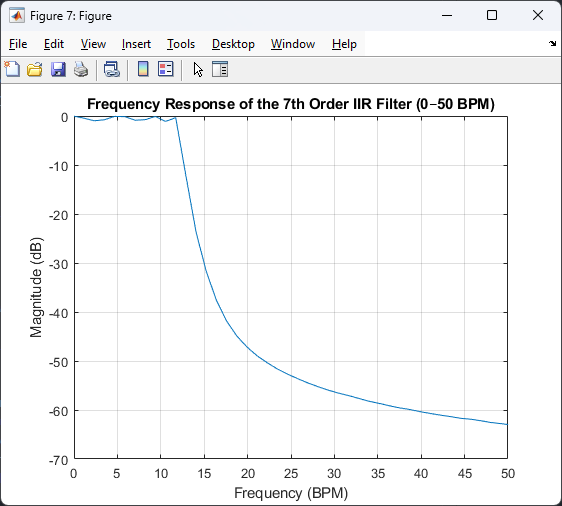
\includegraphics[width=\linewidth]{7thOrderIIRFrequency.png}
    \caption{7th Order Chebyshev Filter Impulse Response}
    \label{fig:7th_cheby_high_freq}
\end{figure}

Finally a 5th order Chebyshev Bandpass filter, with a ripple of 1.0 dB, with a low corner frequnecy of 12 BPM, and a high corner frequency of 25 BPM was designed. Using the imnpulse response as the input the frequnecy was plotted.

\begin{figure}[H]
    \centering
    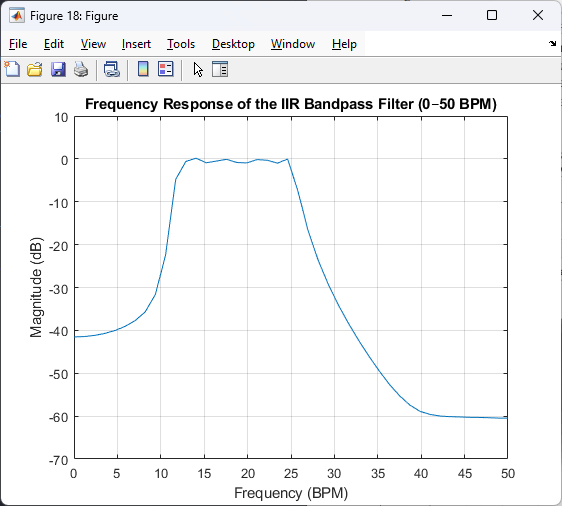
\includegraphics[width=\linewidth]{BandpassSOSFrequency.png}
    \caption{7th Order Chebyshev Filter Impulse Response}
    \label{fig:5th_cheby_band_freq}
\end{figure}

The result of this shows that the bandpass frequency range was met. This can be seen because as the the frequency reaches 12 BPM, the signal is passed through, and as the frequency reaches pas 25 BPM, the signal is attenuated.

This filter was then tested with a test vector of sinusoidal signals at 5, 10, 15, 20, 30, and 70 BPM. The output was analyzed in MATLAB to confirm that the filter passed the desired frequencies while attenuating others.

The results showed that the filter effectively isolated the desired frequency range, confirming its design specifications.

\begin{figure}[H]
    \centering
    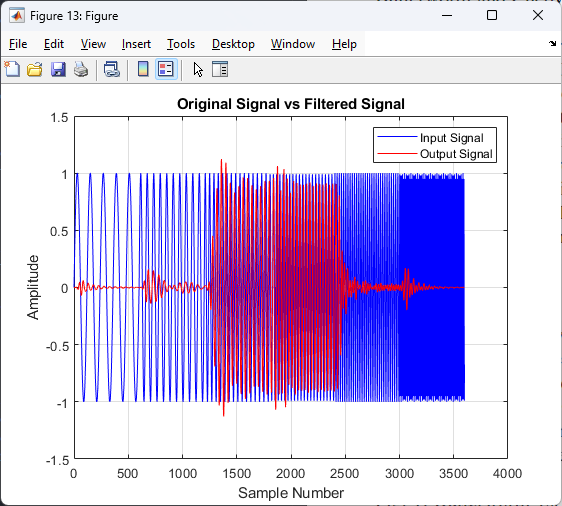
\includegraphics[width=\linewidth]{plot7a.png}
    \caption{Bandpass Filter}
    \label{fig:5th_cheby_band_freq_final}
\end{figure}

Overall, the analysis confirmed that each filter performed according to its theoretical design. The Butterworth filter provided a smooth, ripple-free passband, while the Chebyshev filters demonstrated the expected sharper roll-off with controlled ripple. The direct form implementation revealed the instability issues that can arise with high-order filters, emphasizing the importance of using Second Order Sections for practical deployment. The final bandpass filter effectively isolated the desired breathing rate range of 12–25 BPM, and its performance was validated through both impulse response analysis and sinusoidal test vectors. These results underscore the accuracy of the MATLAB-based filter design and the effectiveness of the Arduino implementation.

\section{Conclusion}
This lab successfully explored the design, implementation, and evaluation of various IIR filter types using both theoretical tools and embedded hardware. The transition from direct form to Second Order Sections proved crucial for maintaining stability in high-order designs, highlighting an important real-world consideration in digital signal processing. By combining MATLAB's powerful design tools with Arduino's real-time capabilities, this lab reinforced key concepts in filter design and demonstrated their practical applications for physiological signal processing such as respiratory rate detection.

\end{document}
